% Proposal (3.5p)
\section{Motivating Example: The Filling Station Advisor}
\label{sec:case_study}

In this paper, we use a case study of a filling station advisor application. Filling station here refer to a place where the car can be refueled or recharged (gas station/petro or charge station). The main goal of the filling station advisor is to give direction to a vehicle driver about nearby filling stations that can be reached conveniently. By convenient we mean that certain conditions for the chosen station have to be fulfilled as well as user preferences are considered. Examples of conditions are: fuel is compatible with the vehicle; station is located inside the vehicle distance-to-empty. Examples of users preferences are: low price, low number of stops, small deviation from an actual route, and station reputation.

In this work, we will focus on the challenge of handling the computing variability when developing such application. To maximize the utility, the filling station advisor should be able to run in a broad range of devices like smart-phones and car navigation systems. Each of such devices can have a different set of resources that can be used to find a convenient filling station according to the user preferences. For example, in a scenario where a human driver is using the application with a smart phone, we could use the GPS resource to track the position and the distance since the last refueling; the Internet connection to find nearby filling stations; the device text-to-speech engine to create a voice message to alert the driver when he is passing by a convenient filling station. In another scenario, in which the application is running in on-board computer of an Internet connected self-driving car, we could use a more precise distance-to-empty data from on-board computer, and replace the text-to-speech notification with a system call to the vehicle self-driving system advising the next filling station stop.

The filling station advisor's main goal can be refined into the following five goals, each one with its own computing resources requirements:

\begin{description}
  \item[Identify Vehicle Position:]
  the system should identify the vehicle position using an available positioning system. To fulfil such goal, a GPS or cell antenna triangulation could be used.

  \item[Assess Distance to Empty:]
  the system should make use of the best available data about the vehicle distance to empty. It could be: access a standard or proprietary interface within the vehicle that provides the data directly as calculated by the on-board computer; use an interface to access data about fuel level and mileage average and calculate the distance to empty; use user input about tank capacity, vehicle mileage, and keep track of distance traveled since the last time the tank was felt completely.

  \item[Recover information about nearby filling stations:]
  the system should recover information about nearby filling stations by: querying available services on the Internet, if connection and servers are available. Otherwise, the system should use previously cached results.

  \item[Decide on the most convenient filling station:]
  Based on position, distance to empty and nearby gas stations, the application should try maximize some user preference, it being low cost, low number of stops, prioritize an automotive fuel brands or gas station reputation.

  \item[Notify Driver:] the application should decide when and how to notify the driver with advices on when to stop in a filling station. The notification could be integrated with an active navigation system if such an interface exists; otherwise it should notify the driver using text-to-speech engine, a pre-recorded voice audio, or on-screen notification.

\end{description}

\begin{figure}[!htb]
 \centering
 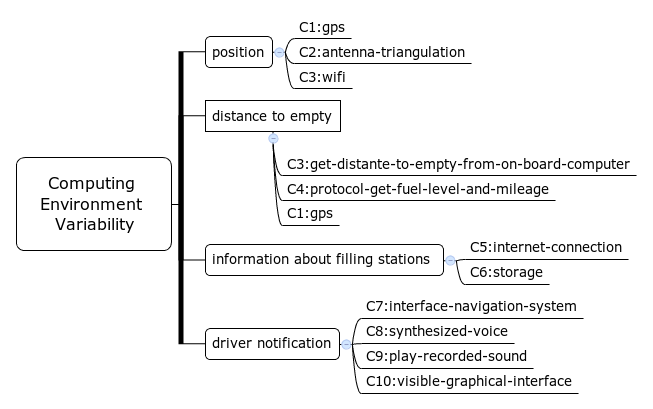
\includegraphics[width=\linewidth]{case_study/variability}
 \caption{Variability in the Computing Environment}
\label{fig:variability}
\end{figure}

\begin{figure*}[!htb]
 \centering
 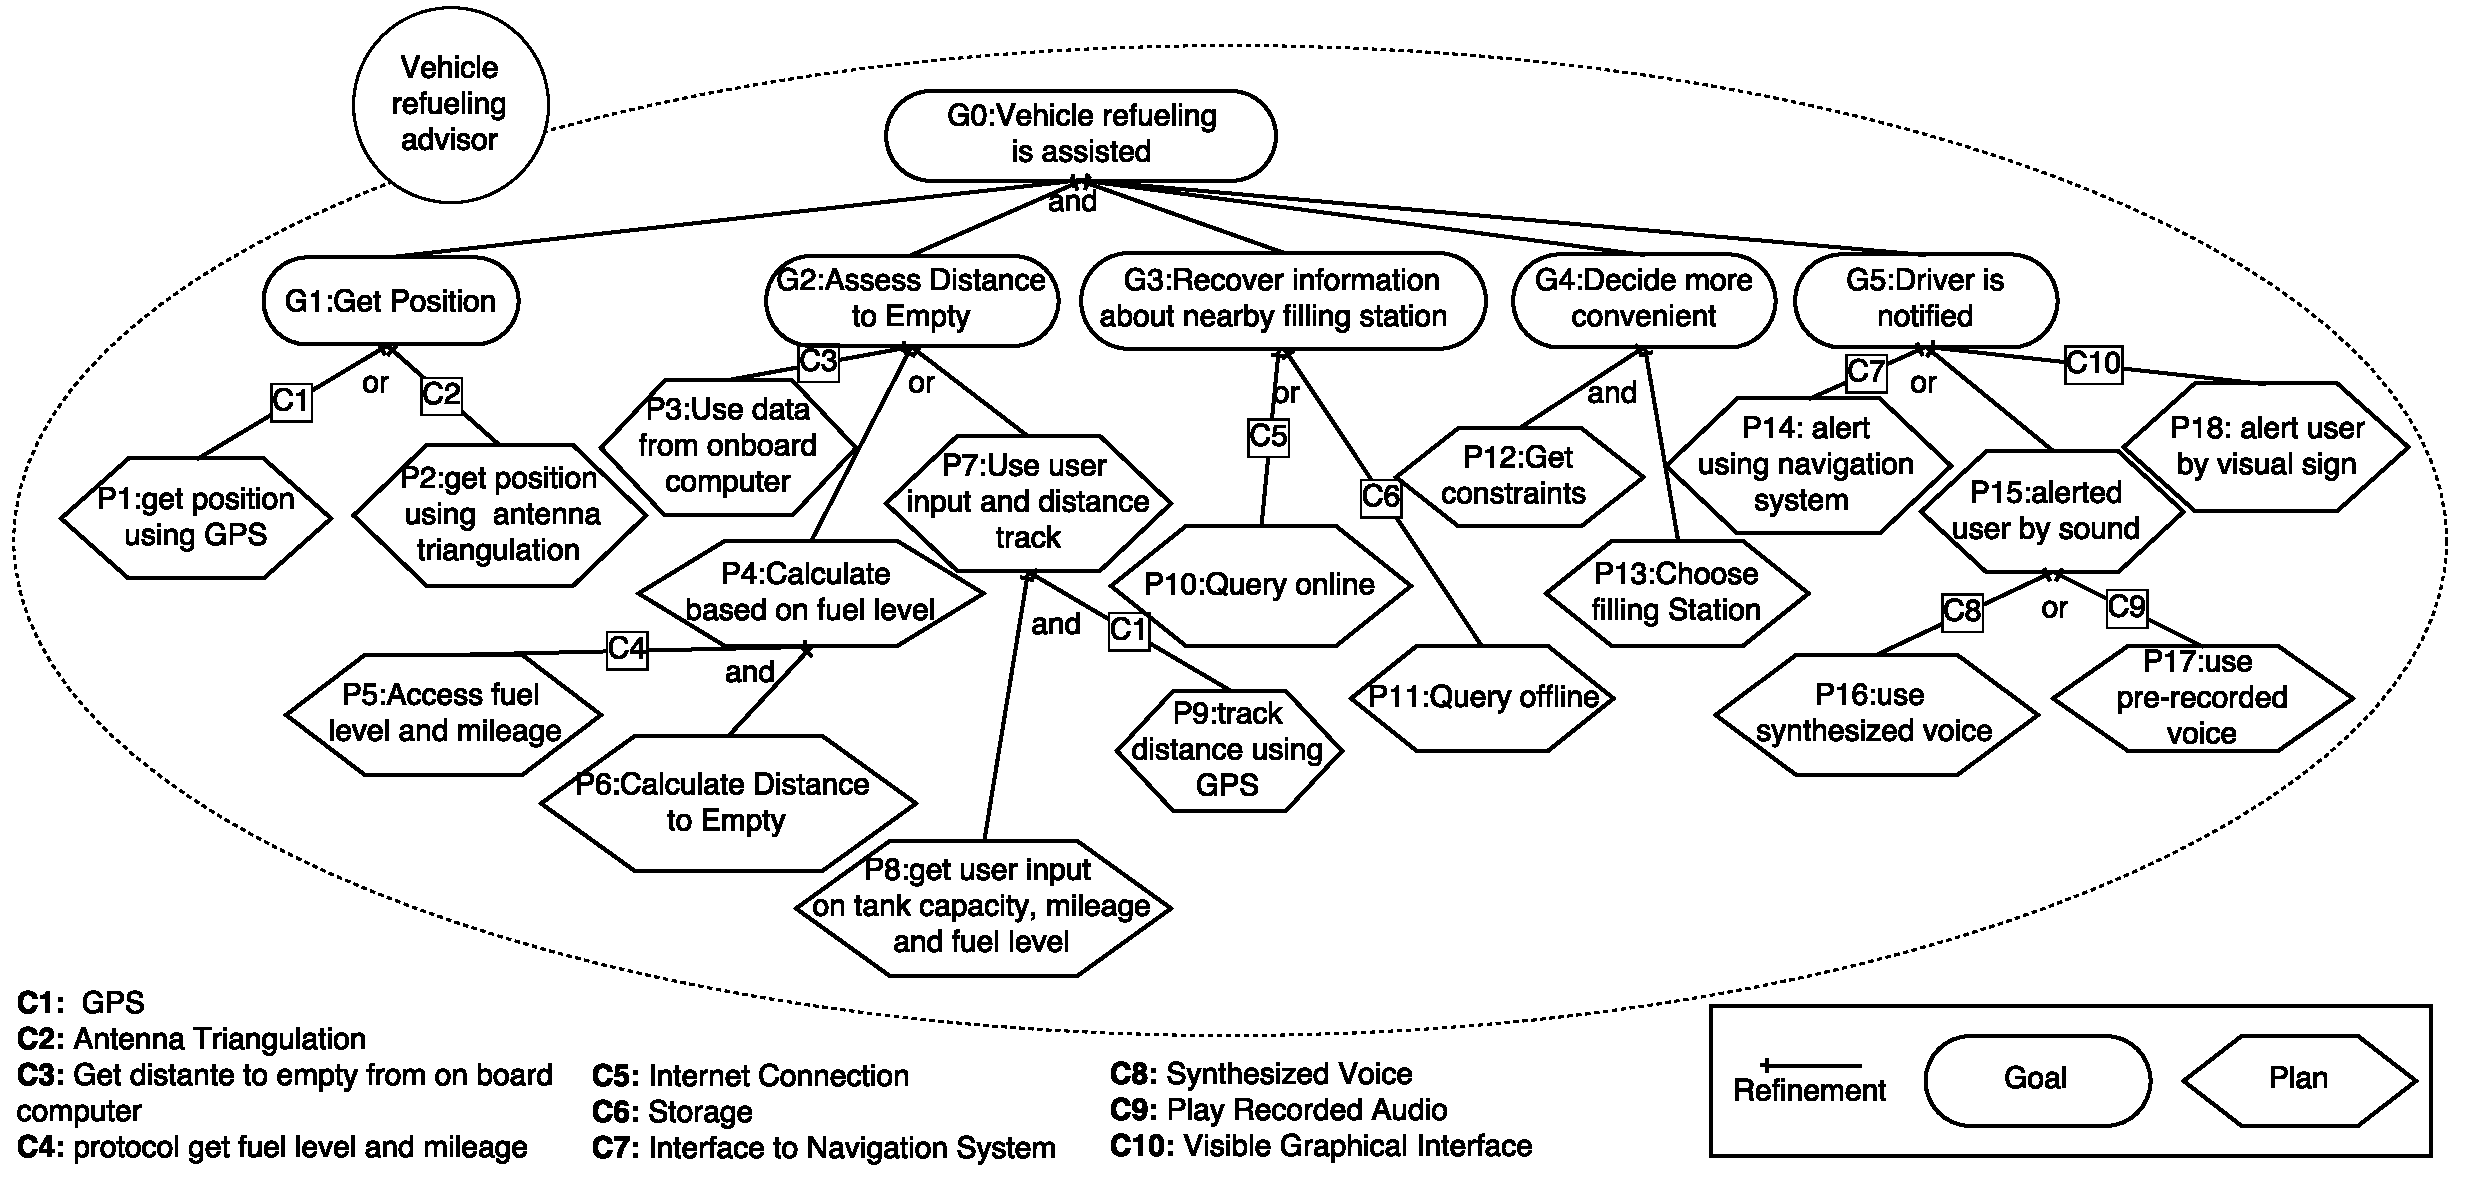
\includegraphics[width=\linewidth]{case_study/goal_model_filling_station_advisor}
 \caption{CGM of the filling station advisor}
\label{fig:goal_model_filling_station_advisor}
\end{figure*}
